
\documentclass[submit]{ipsj}
%\documentclass{ipsj}

\usepackage[dvipdfmx]{graphicx}
\usepackage{latexsym}
\usepackage{listings}

\lstset{
  frame=single,
  numbers=left,
  tabsize=2
}

\def\Underline{\setbox0\hbox\bgroup\let\\\endUnderline}
\def\endUnderline{\vphantom{y}\egroup\smash{\underline{\box0}}\\}
\def\|{\verb|}

\setcounter{巻数}{59}
\setcounter{号数}{1}
\setcounter{page}{1}


\受付{2020}{5}{10}
\再受付{2015}{7}{16}   %省略可能
\再再受付{2015}{7}{20} %省略可能
\再再受付{2015}{11}{20} %省略可能
\採録{2016}{8}{1}




\begin{document}


\title{Webアプリケーションを安全にする
\\新しいフレームワークの機能}

\etitle{A New Framework Feature to Secure Web Applications}

\affiliate{KU}{九州大学システム情報科学府\\
Graduate School and Facility of Information Science and Electrical Engineering, Kyushu University}
\affiliate{RIIT}{九州大学情報基盤研究開発センター\\
Research Institute for Information Technology, Kyushu University}

\author{久保田 康平}{Kohei Kubota}{KU}[kouhei.kubota@icloud.com]
\author{小出 洋}{Hiroshi Koide}{RIIT}

\begin{abstract}
Webアプリケーション開発者が実装するコードを実行時に自動的に解析し,必要ならば修正する機能をWebアプリケーションフレームワークに持たせることを提案し,実装して評価を行う.
アプリケーション開発者は常に完全にセキュアなコードを書くことはできず,脆弱性が残る実装を残してしまうことがある.
そのため,実装されたコードを自動的に解析し,修正する機能はフレームワークが持つべき機能のひとつである.
提案手法を実証し評価を行った結果,この機能は実装されたコードの脆弱性を一部修正でき,レスポンスタイムは提案手法を適用しなかった場合とほとんど変わらないことを確認した.
実装された修正関数の蓄積は将来のアプリケーションのセキュリティの向上に寄与できるものである.
\end{abstract}


\begin{jkeyword}
セキュアプログラミング,Webセキュリティ,Webアプリケーションフレームワーク
\end{jkeyword}

\begin{eabstract}
We propose, implement, and evaluate a web application framework that automatically analyzes the code implemented by web application developers and modifies the code if necessary.
Developers can't always write perfectly secure code, leaving implementations that remain vulnerable.
Therefore, the ability to automatically analyze and modify the implemented code is one of the features that a framework should have.
We demonstrated and evaluated the proposed method and confirmed that this feature can fix some vulnerabilities in the implemented code.
In addition, it was confirmed that the response time was almost the same as the case without the proposed method.
An accumulation of implemented modification functions will contribute to improve the security of future applications.
\end{eabstract}

\begin{ekeyword}
secure programming, web security, web application framework
\end{ekeyword}

\maketitle

%1
\section{はじめに}
本論文は,Webアプリケーションのセキュリティ機能向上を目的にしている.
その目的の達成のために,アプリケーション開発者が実装したプログラム中の関数や引数を解析し,実行時にその関数に脆弱性があった時には修正することができるWebアプリケーションフレームワークを提案,実装し評価する.
%WAFや単なるWebフレームワークとの比較,多層防御の考え方における本手法の位置付け

Webアプリケーションフレームワークはアプリケーション開発者に,Webアプリケーションのセキュリティを向上させる機能を提供している.
したがって,アプリケーション開発者はWebアプリケーションフレームワーク上の関数を用いることで,脆弱性が低減されたWebアプリケーションを実装できる.
しかし,アプリケーション開発者は時としてWebアプリケーションフレームワークを利用して,脆弱性があるアプリケーションを実装することがある.
アプリケーション開発者が,Webアプリケーションフレームワークが提供する関数やモジュールを,適切に利用できないことがあるためである.
これはアプリケーション開発者が実装したプログラム中の脆弱性を,Webアプリケーションフレームワークが解消できないという問題である.
この問題は,もし全ての脆弱性への対策を提供しているWebアプリケーションフレームワークが存在し,そのフレームワークをアプリケーション開発者が利用しても,脆弱性があるアプリケーションを開発しうることを意味している.

また,アプリケーション開発者に対するWebアプリケーションフレームワークの学習コストの高さも問題である.
Webアプリケーションフレームワークは,それぞれが独自の仕様をアプリケーション開発者に提供しているので,アプリケーション開発者は異なるフレームワークを利用する際にそれぞれのフレームワークが提供しているシステムの仕様を知っている必要がある.
セキュリティについても同様で,アプリケーション開発者の知識不足や誤解が,脆弱性があるWebアプリケーションを実装する要因になる.

% 静的なコードの解析との比較(本手法が動的な解析であること)
Webアプリケーションのセキュリティを高める手法として,アプリケーションを解析による脆弱性の検出がある.
解析手法は静的解析と動的解析の二つに分類される.
静的解析は,アプリケーションのソースコードを調べることで脆弱性を発見する解析手法である.
アプリケーションを実行することなく,脆弱性を発見できるため,テストデータやテスト環境が必要ないため,早期に脆弱性を発見することが可能である.
しかし,アプリケーションを実行せずにソースコードのみで解析するため,発見できる脆弱性の種類は少なく,また誤検知が多い.
一方,動的解析はアプリケーションに対する入力とその出力から,脆弱性を検出する解析手法である.
動的解析はアプリケーションを実行して脆弱性を検出するため,誤検知が少ないことが利点であり,また認証や認可などに関する広範な脆弱性を検出することが可能である.
Webアプリケーションフレームワークの中には,動的解析を行う環境を提供するものがある.
アプリケーション開発者がテストデータを作成し,そのデータを入力として,出力が正しいかをフレームワークが自動で行うことで,アプリケーションが正しく機能するかを解析することができる.
しかし,アプリケーション開発者はテストデータを作る必要があり,開発時間や作業量が増加する要因になる.

Webアプリケーションの脆弱性を低減する手法の一つとして,Webアプリケーションファイアウォール(WAF)\cite{waf}を利用することがあげられる.
WAFは,クロスサイトスクリプティング(XSS)やSQLインジェクション(SQLi)などのWebアプリケーションの脆弱性を利用する攻撃からWebアプリケーションを保護するシステムである.
Webアプリケーションとクライアント間の通信を監視し,攻撃である通信を検出した時,その通信を遮断したり修正したりする.
WAFは,アプリケーションを修正することなく,脆弱性に対する攻撃を低減することができるため,アプリケーションを直接修正できない状況の時に,特に有効である.
一方でWAFは,アプリケーションを修正しないため,実装における防御の根本的な解決にはなっていない.
攻撃の対策のためには,アプリケーションそのものを修正する必要がある.
また,WAFでは対策しづらい攻撃が存在する.
WAFはリクエスト内の特殊文字によって攻撃かどうかを判断するが,主に認証や認可について脆弱性があるWebアプリケーションに対する攻撃は,特殊文字を利用することなく行うことができるため,WAFでは防御しづらい.

これらの問題を解決するために,本論文ではアプリケーション開発者が実装したソースコードを修正し,必要に応じて修正するWebアプリケーションフレームワークが備えるべき機能を提案する.
アプリケーションの実行時に,アプリケーション開発者が実装したコールバック関数中に存在する脆弱な関数を安全な関数に変換したり,その関数の引数に対して入力検証を行う関数を自動で挿入したりすることで,脆弱性を低減するものである.
この機能はアプリケーション開発者が,脆弱性の解析のために追加の実装を行うことなく,アプリケーションを動的に検証する関数や変数を追加することができる.
% 何ができるようになるか?認証、認可
この機能により,これまでのWebアプリケーションフレームワークやWAFでは対策がしづらかった,管理者しか利用できない関数やデータについての脆弱性の対策をフレームワークが行うことができる.
権限が必要なメソッドをコールバック関数内で呼び出した時に,フレームワークが,リクエスト情報を利用して,正しい権限を持っているかどうかを検証するメソッドをコールバック関数内に追加してくれることが可能だからである.
また,動的な解析が可能であるため,静的な解析より広範なセキュリティ機能を実装できる.
加えて,この機能は実行時にアプリケーションを自動で修正するので,アプリケーション内の脆弱性を直接修正できる点でWAFとは異なる.

このフレームワークの機能は,Python\cite{py}を用いて実装された.
Pythonは関数を引数や戻り値に取れる言語であることから本論文の手法を実装するのに適した言語の一つである.
このフレームワークは,具体的には4つの工程によりプログラムを修正する.
まず活動中のオブジェクトから,アプリケーション開発者が実装した関数のソースコードを取得する.
アプリケーション開発者が実装した関数とは,クライアントのリクエストヘッダに基づいて呼び出されるコールバック関数である.
このフレームワークは,コールバック関数を実行可能な形式で受け取り,その関数のソースコードを組み込み関数を利用してフレームワークに格納する.
次にそのソースコードを抽象構文木\cite{compiler}に変換する.
その後,その構文木を修正する.
そして最後に実行可能なオブジェクトに変換しなおすことで,ソースコードを修正する.
この工程により,アプリケーション開発者が実装した関数はフレームワークに修正されたのちに,フレームワークに格納される.

検証として,このWebアプリケーションフレームワークの機能を利用して,アプリケーション開発者が実装したコードに脆弱性があるWebアプリケーションを実装して評価を行った.
結果として,組み込み関数によってできたSQLi脆弱性を,フレームワークが自動で修正できることがわかった.またこれ以外の脆弱性を除去する機能も実現できることを議論した.

%2
\section{関連研究}
Webアプリケーションフレームワーク上で実装したソースコードを自動的に解析する技術として,\cite{rubyx}がある.
この論文は,Webアプリケーションフレームワーク上のソースコードをセキュアにするという目的と,そのソースコードを自動で解析することができる点で類似している.
この論文ではシンボリック実行を利用して,到達可能性を調べることにより脆弱性を探索し,脆弱性と判定されれば,アプリケーション開発者に警告を返す.
このシステムの長所は,既存のWebアプリケーションフレームワークであるRuby-on-Rails\cite{rails}のソースコードの解析を行うことができることである.

抽象構文木を用いたセキュリティに関する研究として\cite{ast_js}があげられる.
この論文は抽象構文木の特徴を利用して難読化されたJavaScriptの悪性を判断する手法を提案している.
抽象構文木はプログラム内の無意味な部分を除去することができるので,プログラムの意味を抽出しやすいことと,抽象構文木を実装するために,動的な解析を必要としないので高速な点が長所である.
抽象構文木は,即時性を求められるWebプログラミングの解析に向いた手法だと言える.

%3
\section{提案手法}
コールバック関数を修正する際,コールバック関数は修正機能を実装するWebアプリケーションフレームワークの開発者にとって編集しやすいことが望ましい.
もしコールバック関数を直接修正しようとすると,Pythonの実行可能なオブジェクトはバイナリデータであるため,バイナリである関数を引数にとって,それを編集する関数をフレームワーク上に実装する必要がある.
これは編集を行いやすいとは言えない.
このフレームワークはコールバック関数の修正を簡単にするために,コールバック関数の抽象構文木を修正する.
抽象構文木とは,プログラムを実行可能なバイナリのコードにする過程で得られる中間コードである.
構文木の構成要素はノードで表され,それぞれの要素はプログラムのコードオブジェクトに影響がある要素である.
抽象構文木は,コードオブジェクトにとって意味がない部分をソースコードから取り除いているため,プログラムの意味を修正しやすい特徴がある.
また,構文木のノードにはコード生成のルールが似ている演算子をひとまとめにした型が存在するため,型による条件一致によって修正する対象を見つけやすいという特徴がある.

なお開発者の呼称の区別として,この章以降Webアプリケーションフレームワークを利用して,コールバック関数を実装する開発者をWebアプリケーション開発者,もしくはアプリケーション開発者とし,
フレームワークを実装して,コールバック関数を修正する関数をフレームワーク上に実装する開発者をWebアプリケーションフレームワーク開発者,またはフレームワーク開発者と区別する.
%3.1
\subsection{デコレータ}
このフレームワークはデコレータ\cite{decorator}を利用してアプリケーション開発者が抽象構文木を修正する関数を実装し,コールバック関数に適用する.
デコレータとは,ソースコードの可読性をあげることができるようにする関数を修正する関数の表現方法である.
以下の二つのコード例は,デコレータを利用したソースコードと,それと同じ意味を持つソースコードである.
\begin{lstlisting}[language=python]
@decorator
def func():
  ...
\end{lstlisting}

\begin{lstlisting}[language=python]
def func():
  ...
func = decorator(func)
\end{lstlisting}

\subsection{コールバック関数の修正}
このフレームワークは,コールバック関数を修正する関数をフレームワーク内に実装することで,脆弱性を修正することができる.
%説明(astの修正関数を追加する手法)
この修正関数は,コールバック関数の抽象構文木を引数として受け取り修正を行う.
抽象構文木の修正は,構文木中の修正するノードの探索とその修正によって行われる.
ノードを再帰的に探索して,修正関数で定義した条件が一致するものを見つける.
この条件はノードの属性や名前などである.
そして条件を満たすノードが見つかった際に,ノードの一部を修正することで,コールバック関数を修正することができる.
抽象構文木は複数回修正することが可能であり,一つの修正関数内で複数回修正することも複数の修正関数を利用して構文木を修正することも可能である.
%新しい脆弱性をハンドルする仕組みを入れるとした時の手法
複数の修正関数を利用して脆弱性を対策することが可能であるため,コールバック関数内に新しい脆弱性が見つかった時,新たに修正関数を実装すれば,コールバック関数と今まで実装した修正関数を変更せずに脆弱性の影響を低減できる.
%図


\begin{figure*}[tb]
\begin{centering}
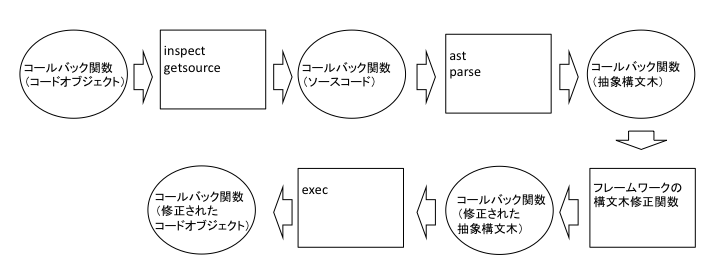
\includegraphics[width=17.6cm]{./figures/easy_diagram.png}
\caption{コールバック関数を修正する工程の簡易図.}
\ecaption{Simplified diagram of the process to fix a callback function.}
\label{fig:fixer}
\end{centering}
\end{figure*}

また,アプリケーション開発者がコールバック関数の修正関数を実装し,コールバック関数を修正することも可能である.
この手法の利点は同一の脆弱性への対策をコールバック関数に追加する際,修正関数に実装した条件から機械的に修正するので,対策漏れを減らすことができるという点である.
以下のような実装を行うことで,コールバック関数を修正させることができる.
\begin{lstlisting}[language=python]
@app.funcFixer.addNodeFixer
def rewriteNode(node):
    new_node = Rewrite().visit(node)
    return new_node

@app.route("^/$", "GET")
@app.funcFixer.fix("rewriteNode")
def index(request):

    return "Hello"
\end{lstlisting}
このソースコードは二つの関数とそれらに関わるデコレータから構成される.
1行目から4行目がアプリケーション開発者が実装できるコールバック関数の抽象構文木を修正する関数であり,5行目から10行目がコールバック関数である.
1行目のapp.funcFixer.addNodeFixerは,抽象構文木を修正する関数をフレームワーク内に格納するメソッドである.
修正関数はaddNodeFixerメソッドによってフレームワークに渡され,関数名をキー,コードオブジェクトバリューとした辞書形式で格納される.
2行目の引数であるnodeはフレームワークから与えられるコールバック関数の抽象構文木である.
3行目のRewriteはPythonが提供する抽象構文木を修正するヘルパーであるast\cite{AST}モジュールのうち,ast.NodeTransformerの子クラスであり,そのインスタンスの生成している.
このRewriteクラスに,抽象構文木を修正する条件や修正する方法を記述する.
また,visitメソッドは抽象構文木の探索と修正を行うメソッドである.

コールバック関数の実体は,8行目から10行目までである.
8行目の引数requestはリクエスト情報をコールバック関数内で利用しやすいようにフレームワークが整形したものである.
6行目は,コールバック関数をフレームワークに格納するデコレータで,第一引数がパスの正規表現,第二引数がリクエストメソッドである.
この二つの引数を満たすリクエストが送信されると,コールバック関数が呼ばれる.
7行目がコールバック関数を修正するデコレータである.
修正関数の名前を受け取り,フレームワークに格納された関数を利用してコールバック関数を修正する.

%4
\section{実装}
\figref{fig:fixer}は,このフレームワークがコールバック関数を修正するために必要な工程を表している.

\figref{fig:fixer}に示す通り,Webアプリケーション開発者が実装したコールバック関数を抽象構文木に変換して,解析・修正するために4つの工程が必要である.
一つ目が,コードオブジェクトからテキストを受け取ることである.
これは,Pythonが提供している抽象構文木に対するヘルパーであるastモジュールが,実行可能なバイナリデータを直接抽象構文木に変換できないためである.
コードオブジェクトからテキストを受け取るために,inspect\cite{inspect}モジュールを利用する.
inspectモジュールは,活動中のオブジェクトから情報を取り出すモジュールである.
このモジュールのうち,getsourceメソッドを利用して関数のソースコードを取得する.
getsourceメソッドは,ソースコードの該当部分をテキストファイルとして読み込むことで,ソースコードを取得する.
動的に実行したコードオブジェクトから,ソースコードを取得しようとするとOSErrorを起こすことがあるため注意が必要である.
特に,フレームワークによって修正された関数は動的に生成された関数であるため,ソースコードを取得できない.
%テキストを構文木に変更する

二つ目に,関数のソースコードを抽象構文木に変換する.
ソースコードを構文木に変更できる形に整形する.
具体的にはソースコードの先頭にあるインデントの分だけ各行のインデントを取り除く.
これはソースコードの先頭にインデントがある状態では,抽象構文木を作成できないためである.

%構文木を解析,修正する
三つ目は構文木を解析・修正する工程である.
この工程では,まず抽象構文木からコールバック関数のデコレータ部分を取り除く.
これは,デコレータの一部に活動中のオブジェクトを元にソースコードを探す処理があり,動的に生成されたコードオブジェクトのソースコードを取得しようとしてエラーを起こすためである.
この工程でデコレータを取り除く理由は,フレームワークのデコレータだけを取り除くようにするためである.
抽象構文木を利用すると,モジュール名とメソッド名からデコレータを取り除くことができるため誤りが少ない.
デコレータを取り除いたのちに,関数の内容を修正する.
この工程はアプリケーションフレームワークで自動的に行われる修正を行い,その後Webアプリケーション開発者が実装した修正を行う.

%構文木からコードオブジェクトを作り,格納する
最後に修正された構文木を活動中のオブジェクトに変換する.
Pythonには抽象構文木を実行可能なオブジェクトに変換するexec\cite{exec}という組み込み関数がある.
この関数を利用してできた関数はデフォルトでは,ローカル変数であるため注意が必要である.

以下の工程を経てコールバック関数は修正され,フレームワーク内に格納される.

%5
\section{実験と結果}
本論文が提案するフレームワークを評価するために,意図的に脆弱なコールバック関数を実装して,その脆弱性をフレームワークが修正できているかを調べる実験を行った.
また,コールバック関数を修正した時としてない時のレスポンスタイムの比較の実験として,cURLコマンドを用いてそれぞれ100回レスポンスタイムを計測し,1リクエストあたりの平均のレスポンスタイムをそれぞれ求めた.
この実験はそれぞれ1度行った.
実験に使用した実装とその結果を以下に示す.
%5.1
\subsection{実験}
この実験は,Python3.7上で実装されている.
アプリケーションは\figref{fig:AppFig}に示す構成である.
\begin{figure}[tb]
\begin{centering}
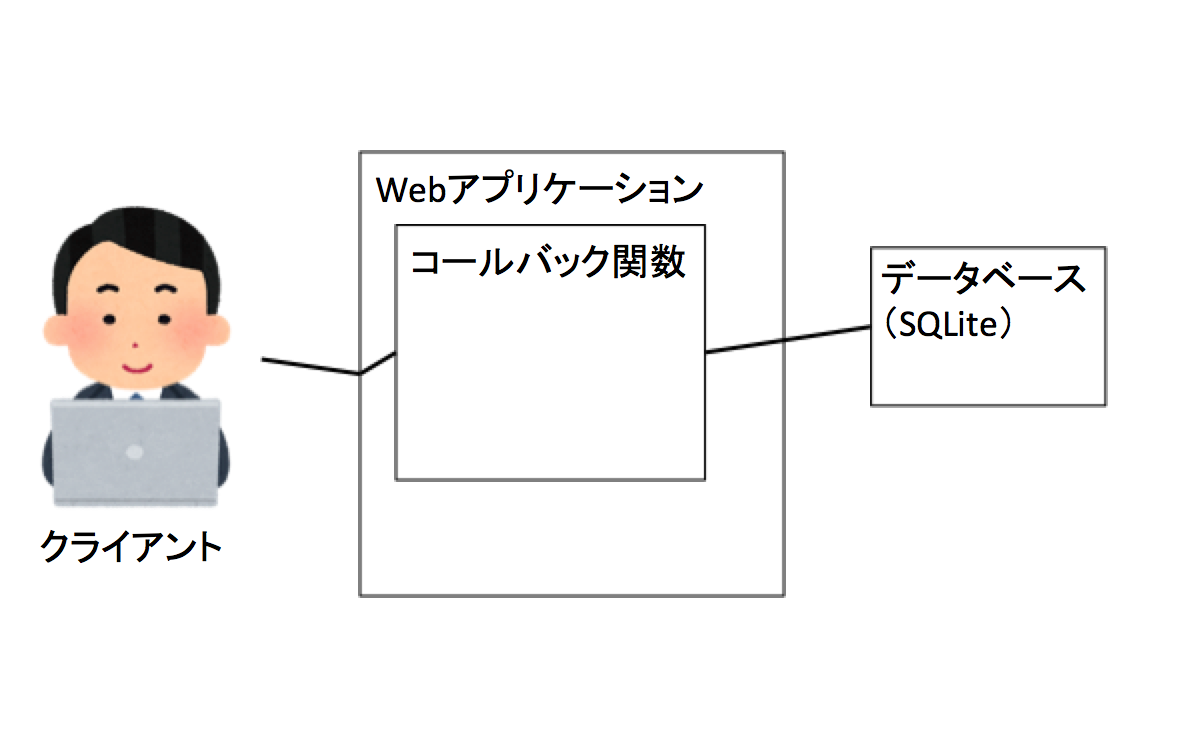
\includegraphics[width=7.0cm]{./figures/sys_strc.png}
\caption{実装したアプリケーションの簡易図.}
\ecaption{Simplified diagram of the implemented application.}
\label{fig:AppFig}
\end{centering}
\end{figure}
実験を行った環境は,OSが MacでOS X El Capitan 10.11.6, CPU が Intel Core i5 (2.95GHz),メインメモリが8GBである.

\subsubsection{コールバック関数の修正}
コールバック関数はデータベースに接続しており,リクエストパラメータからクエリを生成して,データベースに問い合わせ,データベースから受け取った値をブラウザに返す.
クライアントはIDとパスワードを入力するフォームから,これらの情報を入力し,サーバに送信する.
データベースには,IDとユーザ名,パスワードを持つテーブルがある.
IDは,主キーに設定しており同一のIDは存在しないものとする.
このテーブルに対してSQL文を実行し,IDとパスワードが一致するレコードを取得し,そのうちユーザ名とIDをブラウザに返す.

%%%修正
\begin{lstlisting}[language=python]
cur.execute("select * from table1 " + \
"where ID = " + request.params.get["ID"]\
 + " and Password = "\
 + request.params.get("Password"))
\end{lstlisting}

上に示すソースコードは,SQLi脆弱性があるコールバック関数の例のうちの一部である.
cur.executeというSQL文を実行させるメソッドを利用して,データベースから情報を取り出す.
この時,クエリを文字列連結によって組み立てて,そのままデータベースに送っている点にSQLiの脆弱性がある.
例えば,IDに'1 or 1 == 1 order by desc;--',パスワードを空白にした入力を行うと,生成されるクエリは,"SELECT * from table1 where ID = 1 or 1 == 1 order by desc;-- and password = "である.
このクエリはパスワード部分をコメントアウトにより,条件にしないため,テーブル内のIDが最も下にあるレコードを取り出すクエリになってしまう.

このような脆弱性に対して,コールバック内のSQL文を実行する関数の引数をエスケープすることで,脆弱性を低減するように修正する関数を実装した.
具体的には,SQLを利用するモジュールを探し出し,そのメソッド名がexecuteである関数を探索し,その引数の内,リクエストパラメータを利用したものを修正する関数を実装した.
引数を修正する際,コールバック関数内の変数がどのリクエストパラメータを利用しているかを代入する時に調べて,リクエストパラメータ部分だけを修正した.

\subsubsection{レスポンスタイムの比較}
ローカル上にコールバック関数を修正する機能を利用したアプリケーションと利用してないアプリケーションを立ち上げ,レスポンスタイムをそれぞれ一度ずつ測定した.
コールバック関数を修正していないアプリケーションと修正したアプリケーションのレスポンスタイムを,cURLコマンドを用いてそれぞれ100回実行して計測して,1リクエストあたりの平均のレスポンスタイムを求めた.



%5.2
\subsection{結果}
結果として,まず一部のコールバック関数を修正し,脆弱性の一部を低減することができることが分かった.
\begin{lstlisting}[language=python]
import sqlite3

@app.route("^/$", "GET")
@app.addNodeFixer("rewriteExecuteArgs")
def func1(request):
    conn = sqlite3.connect("test1.db")
    cur = conn.cursor()
    cur.execute("select * from table1" \
     + "where ID = " \
     + request.params.get("ID") \
     + " and Password = " \
     + request.params.get("Password"))

    data = cur.fetchone()
    conn.commit()
    return "Hello, " + data[1] \
     + ". Your ID is " + data[0]

\end{lstlisting}

このコールバック関数は,リクエストのパラメータからIDとパスワードを取得し,その情報を元にデータベースを検索し,IDとユーザ名をクライアントに返す.
コールバック関数を修正する関数は8行目から12行目を修正した.
具体的には,cur.executeメソッドの引数のうち,request.params.get("ID")とrequest.params["Password"]を,それらをエスケープした変数に差し替えた.

このコールバック関数について以下にソースコードの説明を記述する.
3行目か5行目は,提案手法で説明したデコレータと関数の宣言である.
6行目と7行目でコールバック関数は,データベースと利用できるようにしている,
具体的には,6行目でデータベース内のテーブルに接続しており,7行目でそのテーブルを操作できるようにしている.
8行目のcur.executeメソッドは引数にクエリを取り,そのクエリをSQLで実行する.
10行目のfetchoneメソッドは,SQLの実行結果のうち,最初に取り出されたデータをタプルの形で出力する.
11行目のcommitメソッドはデータベースを更新するメソッドである.
その後,SQLが返した値を整形してクライアントに返している.

下に示す二つ目のソースコードを修正できたことによって,cur.executeメソッドの引数に直接リクエストパラメータが入ってはいない場合でも修正することが可能であることがわかった.
\begin{lstlisting}[language=python]
import sqlite3

@app.route("^/$", "GET")
@app.addNodeFixer("rewriteExecuteArgs")
def func1(request):
    conn = sqlite3.connect("test1.db")
    cur = conn.cursor()

    s1 = "select * from table1"
    s2 = " where ID = {}" \
     + request.params.get("ID")
    s3 = " and Password = {}" \
     + request.params["Password"]
    s4 = s1 + s2 + s3
    cur.execute(s4)
    data = cur.fetchone()
    conn.commit()
    return "Hello, " + data[1] \
     + ". Your ID is " + data[0]

\end{lstlisting}
一つ目とのソースコードの違いは,9行目から15行目である.
一つ目のソースコードは,cur.executeメソッドの引数に直接リクエストパラメータが入っていたが,今回は入っていない.
変数の代入を調査し,リクエストパラメータを利用した変数を利用することで,修正することができることが確認された.

コールバック関数を修正する関数の実装で脆弱性の対策ができる実装例がある一方で,脆弱性を修正できない場合もあった.
それは,ループによってクエリを動的に作成する場合である.
リクエストパラメータをイテレータとし,各処理でイテレータから要素を変数に代入するが,その代入が通常の代入と異なるために,リクエストパラメータを利用していない扱いになっていたからであった.

レスポンスタイムは修正された関数と修正されていない関数の場合で大きく変わらないことが測定から分かった.
結果は,提案手法を使わない場合のレスポンスタイムが4.98ms/req.で,提案手法を適用した場合が5.28ms/req.であったため,オーバーヘッドは6.09\%程度であった.


%6
\section{考察}
実験の結果から,このフレームワークはコールバック関数を修正し,一部の脆弱性を低減させることが確認できた.
今回は,SQLiを修正する関数を実装して実験を行ったが,他の脆弱性に対しても,修正関数を追加で実装することで修正できると考えられる.
例えばコールバック関数の引数や変数,戻り値を監視することで,XSSの対策も可能だと考えている.
コールバック関数の戻り値はレスポンスボディであり,関数の引数と引数を利用した処理,戻り値を監視することで,リクエストのパラメータによってレスポンスボディが構造的に変化していないかを確認することができるからである.
具体例として以下にあげられるような脆弱なコールバック関数の対策が可能だと考えている.
\begin{lstlisting}[language=python]
@app.route('^/$')
def func2(request):
  head = ...
  body = '<body><p>' \
    + request.params['Name'] \
    + '</p></body>'
  html = head + body
  return html
\end{lstlisting}
上記のコードはレスポンスボディであるhtmlをコールバック関数内で作り,そのまま返すコールバック関数である.
変数headはhtmlのhead部分であり,bodyはリクエストのNameパラメータから値を受け取り,htmlに成形している.
この関数は,リクエストのNameパラメータを直接利用しているため,例えばrequest.params['Name']の内容を\textless
script\textgreater
alert('alert')\textless
/script\textgreater
とすると,JavaScriptのalert関数を呼び出してしまう.
この脆弱なコールバック関数に対して,ノードを修正することを考える.
まずrequest.paramsを利用している変数を探す.
上のコード例では,変数bodyが該当する.
その後,これらの変数が代入された変数を探す.
これはコード例では変数htmlである.
そして,戻り値がこれらの変数を利用している場合,リクエストパラメータを最初に利用する変数を変換する.
コード例では,request.params['Name']をbodyに代入する際に,request.params['Name']の特殊文字をエスケープして代入を行うようにノードを変換することで,対策可能である.
今後,修正関数を追加することで,フレームワークが修正できる範囲も広がり,アプリケーション開発者がほとんど意識することなく広範なセキュリティ機能を利用することが可能になると考えている.

また,レスポンスタイムの比較から,オーバーヘッドは6.09\%と,本論文で提案する手法がレスポンスに大きな影響を与えないことが分かった.
修正後の方がレスポンスタイムが少し大きいのは,修正前にはない処理をコールバック関数に追加しているからだと考えられる.
この時間の追加は,コールバック関数をセキュアにするために必要なレスポンスタイムの追加であると考えられる.

このフレームワークには長所がある一方で制限があることも分かった.
その一つが,コールバック関数内で修正すべき箇所を適切に見つけるのが難しいことである.
その理由は,Webアプリケーション開発者によってソースコードの記述に幅があるからである.
フレームワーク開発者が,同じ意味になるソースコードの記述全てに対して,解析・修正する関数を実装するのは難しい.

\subsection{課題}
本論文で提案したWebアプリケーションフレームワークはコールバック関数を自動で修正するので,フレームワークが脆弱性だと判断したら,それがもし脆弱性ではなかったとしても修正されてしまう.
したがって今後,脆弱性を正しく判定するために,修正関数内の判定方法や判定を行いやすくするヘルパーの実装について考察する必要がある.

また,今後,修正関数が増えると,オーバーヘッドも増加すると考えられる.
ゆえに修正関数とそれに伴うオーバーヘッドの関係性について調査する必要がある.

\subsection{今後の展望}
本論文が提案するフレームワークは,コールバック関数を修正する関数をフレームワークで定義しておけば,Webアプリケーション開発者がコールバック関数上で見逃す脆弱性を修正できる,というものである.
この特徴により,コールバック関数に未知の脆弱性に対して,フレームワーク開発者が修正関数を実装すれば,アプリケーション開発者はフレームワークをアップデートをするだけで,脆弱性の対策ができるようになると考えている.
今後,フレームワークに様々なコールバック関数を修正する関数を追加していくことで,現在発見されていない脆弱性を含めた広範なセキュリティ機能を持つWebアプリケーションフレームワークになっていくと考えている.

また本提案手法は単一のコールバック関数に対して,複数の修正関数を適用できるので,脆弱性を複合的に低減できるようになると考えている.
これは,複数のWebアプリケーションフレームワーク開発者が各々の修正関数を定義し,このフレームワーク上に実装を行うことで,フレームワーク開発者ごとの手法を用いて脆弱性を低減できるという長所だと言える.


%7
\section{おわりに}
本論文では,アプリケーションが持つべき機能として,コールバック関数を自動的に解析し,必要ならば修正する機能を提案し,実装したのちに評価した.
この実装と評価からSQLi脆弱性を一部対策できること,その他の脆弱性に関しても修正する関数を実装することによって対策可能であることが分かった.
一方で,この実装は改良が必要なことも分かった.
今後改良をしていくことで,このアプリケーションフレームワークを利用して,セキュアなアプリケーションを簡単に実装できるようになると考えている.


\begin{acknowledgment}
本研究は,国立研究開発法人科学技術振興機構 (JST)の助成を受けている.また,日立システムズとの共同研究の一部である.
\end{acknowledgment}

\begin{thebibliography}{10}
\bibitem{waf}
独立行政法人情報処理推進機構:
Web Application Firewall(WAF)読本改訂第2版第3刷,\\
\urlj{https://www.ipa.go.jp/files/000017312.pdf}%
\refdatej{2020-06-02}

\bibitem{py}
Python Software Foundation:
python,\\
\urlj{https://www.python.org/}%
\refdatej{2020-05-12}

\bibitem{compiler}
Alfred V. Aho, Monica S. Lam, Ravi Sethi, Jeffrey D. Ullman:
{Compilers : principles, techniques, and tools. --2nd ed.},
pp. 41,
Pearson Education, Inc(2006)

%\bibitem{pycompiler}
%Brett Cannon:
%PEP 339 -- Design of the CPython Compiler,
%\urlj{https://www.python.org/dev/peps/pep-0339}%
%\refdatej{2020-05-12}.

\bibitem{decorator}
Python Software Foundation:
用語集,\\
\urlj{https://docs.python.org/ja/3.7/glossary.html\\\#term-decorator}%
\refdatej{2020-05-14}

\bibitem{rubyx}
A. Chaudhuri and J. S. Foster: {Symbolic Security Analysis of Ruby-on-rails Web Applications},
CCS(2010), pp. 585–594.

\bibitem{rails}
Ruby on Rails,\\
\urlj{https://rubyonrails.org/}%
\refdatej{2020-05-14}

\bibitem{ast_js}
神薗雅紀, 西田雅太, 小島恵美, 星澤裕二:{抽象構文木による不正なJavaScriptの特徴点検出手法の提案},
情報処理学会論文誌,Vol. 54, No. 1, pp. 349-356 (2013).

\bibitem{AST}
Python Software Foundation:
ast --- 抽象構文木,\\
\urlj{https://docs.python.org/\\ja/3.7/library/ast.html}%
\refdatej{2020-05-12}.


\bibitem{inspect}
Python Software Foundation:
inspect --- 活動中のオブジェクトの情報を取得する,\\
\urlj{https://docs.python.org/\\ja/3.7/library/inspect.html}%
\refdatej{2020-05-13}

\bibitem{exec}
Python Software Foundation:
組み込み関数,
\urlj{https://docs.python.org/ja/3.7/\\library/functions.html}%
\refdatej{2020-05-13}

\end{thebibliography}

\end{document}
